\documentclass{article}

% Language setting
% Replace `english' with e.g. `spanish' to change the document language
\usepackage[english]{babel}

% Set page size and margins
% Replace `letterpaper' with`a4paper' for UK/EU standard size
\usepackage[letterpaper,top=2cm,bottom=2cm,left=3cm,right=3cm,marginparwidth=1.75cm]{geometry}

% Useful packages
\usepackage{amsmath}
\usepackage{graphicx}
\usepackage[colorlinks=true, allcolors=blue]{hyperref}

\title{CPE301L: Lab 2}
\author{Joshua Knight, Nicky Victoriano}

\begin{document}
\maketitle

\section{Introduction}

In this lab, we are responsible for programming an Arduino to respond to the presses of two buttons. The arrangement of how these two buttons are pressed affects a set of four LEDs. Each button configuration is read as binary to determine which light is activated, and this effect is based off a provided truth table. The purpose of this lab is to understand decoders by creating a makeshift decoder with our Arduino.

\section{Questions}

\subsection{What is a data bus, address bus, and a control bus? How do they differ?}

To understand any of these, it is first important to understand that a bus is a series of conductive lines that allow communication to occur. A \textbf{data bus} carries data both to and from external systems. An \textbf{address bus} carries any address that needs to be called or written. A \textbf{control bus} carries signals such as the clock or read and write lines. All listed buses share the connection of being buses, but \textbf{ these parts differ in functionality} while being necessary for device communication.

\subsection{Why is a decoder needed in most peripheral device configurations?}

A decoder facilitates the access of addresses and data transmission. If peripheral device configurations did not have a decoder, the given device would not be able to identify and communicate with multiple peripherals when an action is performed.

\section{Results}

\subsection{Circuit}

To create our circuit, we set up the ground and power connections between the appropriate rails. Once this was set up, we connected two buttons with pull-down resistors to the ground and connection to pins 2 and 4 of the Arduino, respectively, to send input signals. Then, we used pins 5 through 8 of the Arduino and connected them to 4 LEDs to act as an output signal. Finally, we connected the serial port of our Arduino to the computer so that the program can run and the serial monitor can also receive the output signals to activate the individual lights. The final circuit and button configurations can be found in \textbf{Table \ref{tab:light-configs}}.

\begin{table}[]
    \centering
    \begin{tabular}{|c|c|}
         \hline
            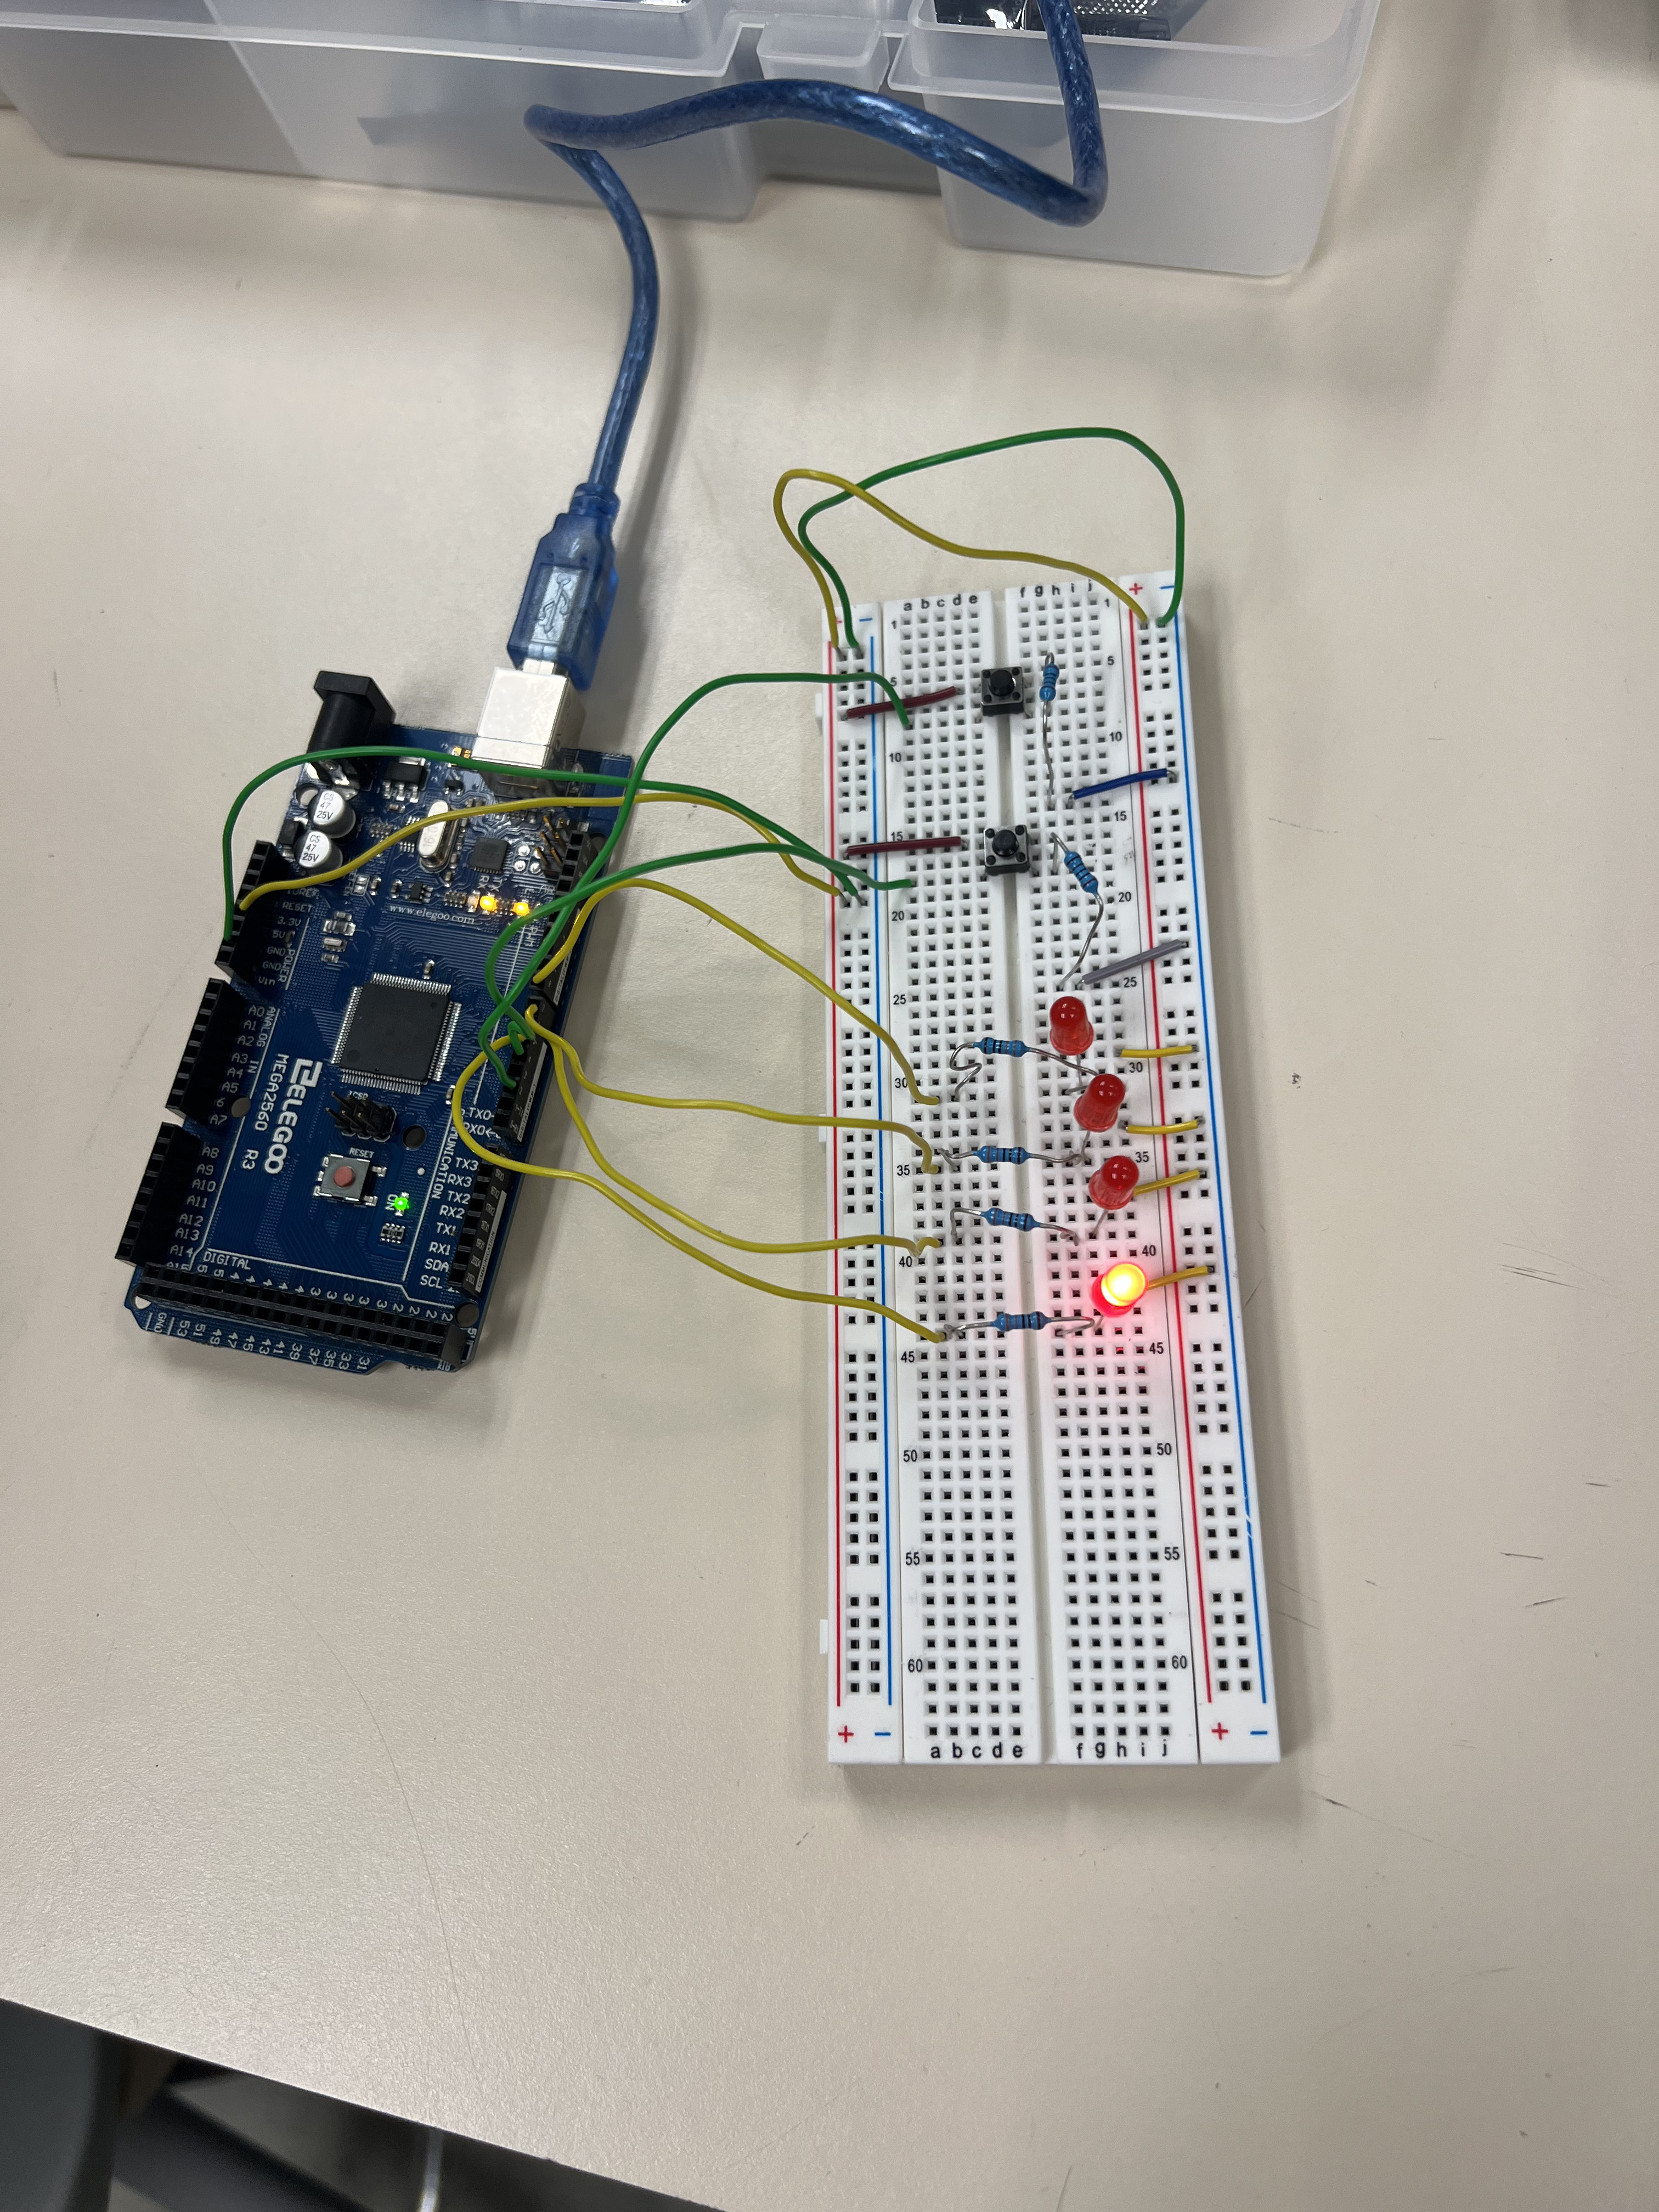
\includegraphics[width=0.28\linewidth]{default.jpg} &
            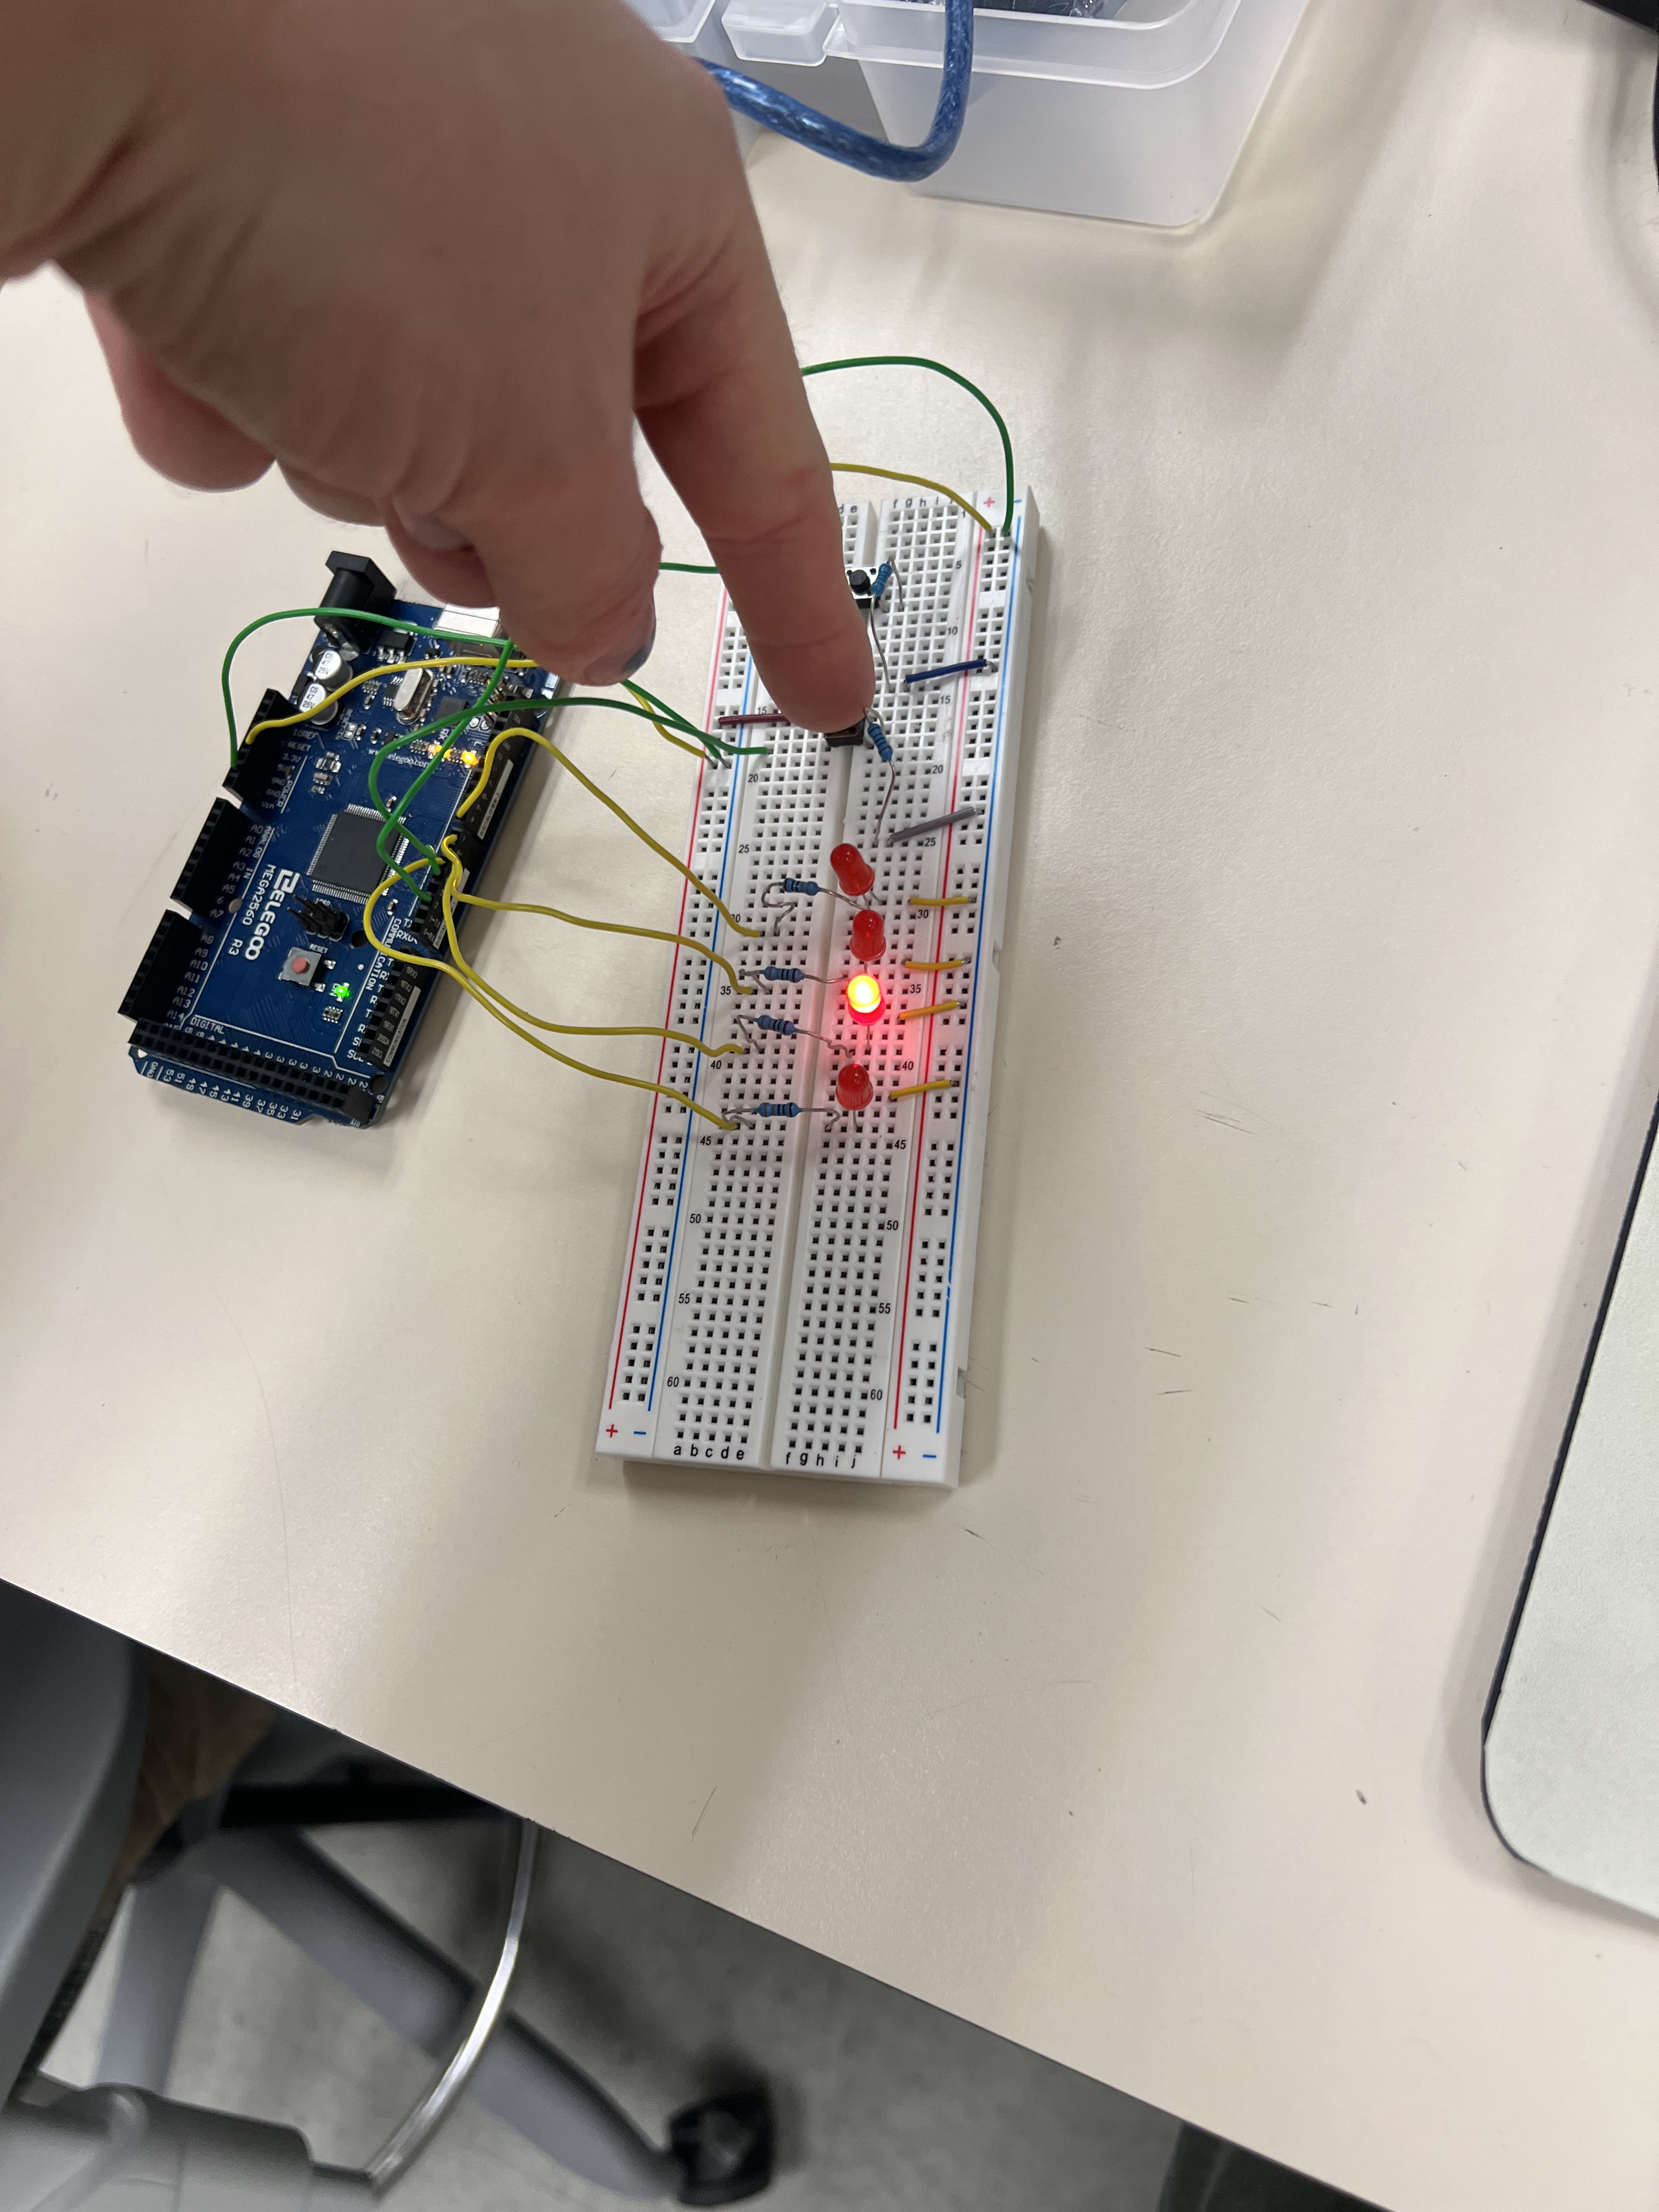
\includegraphics[width=0.28\linewidth]{led-1.jpg}
            \\
            No buttons pressed.&
            Button 1 pressed.
            \\
        \hline
            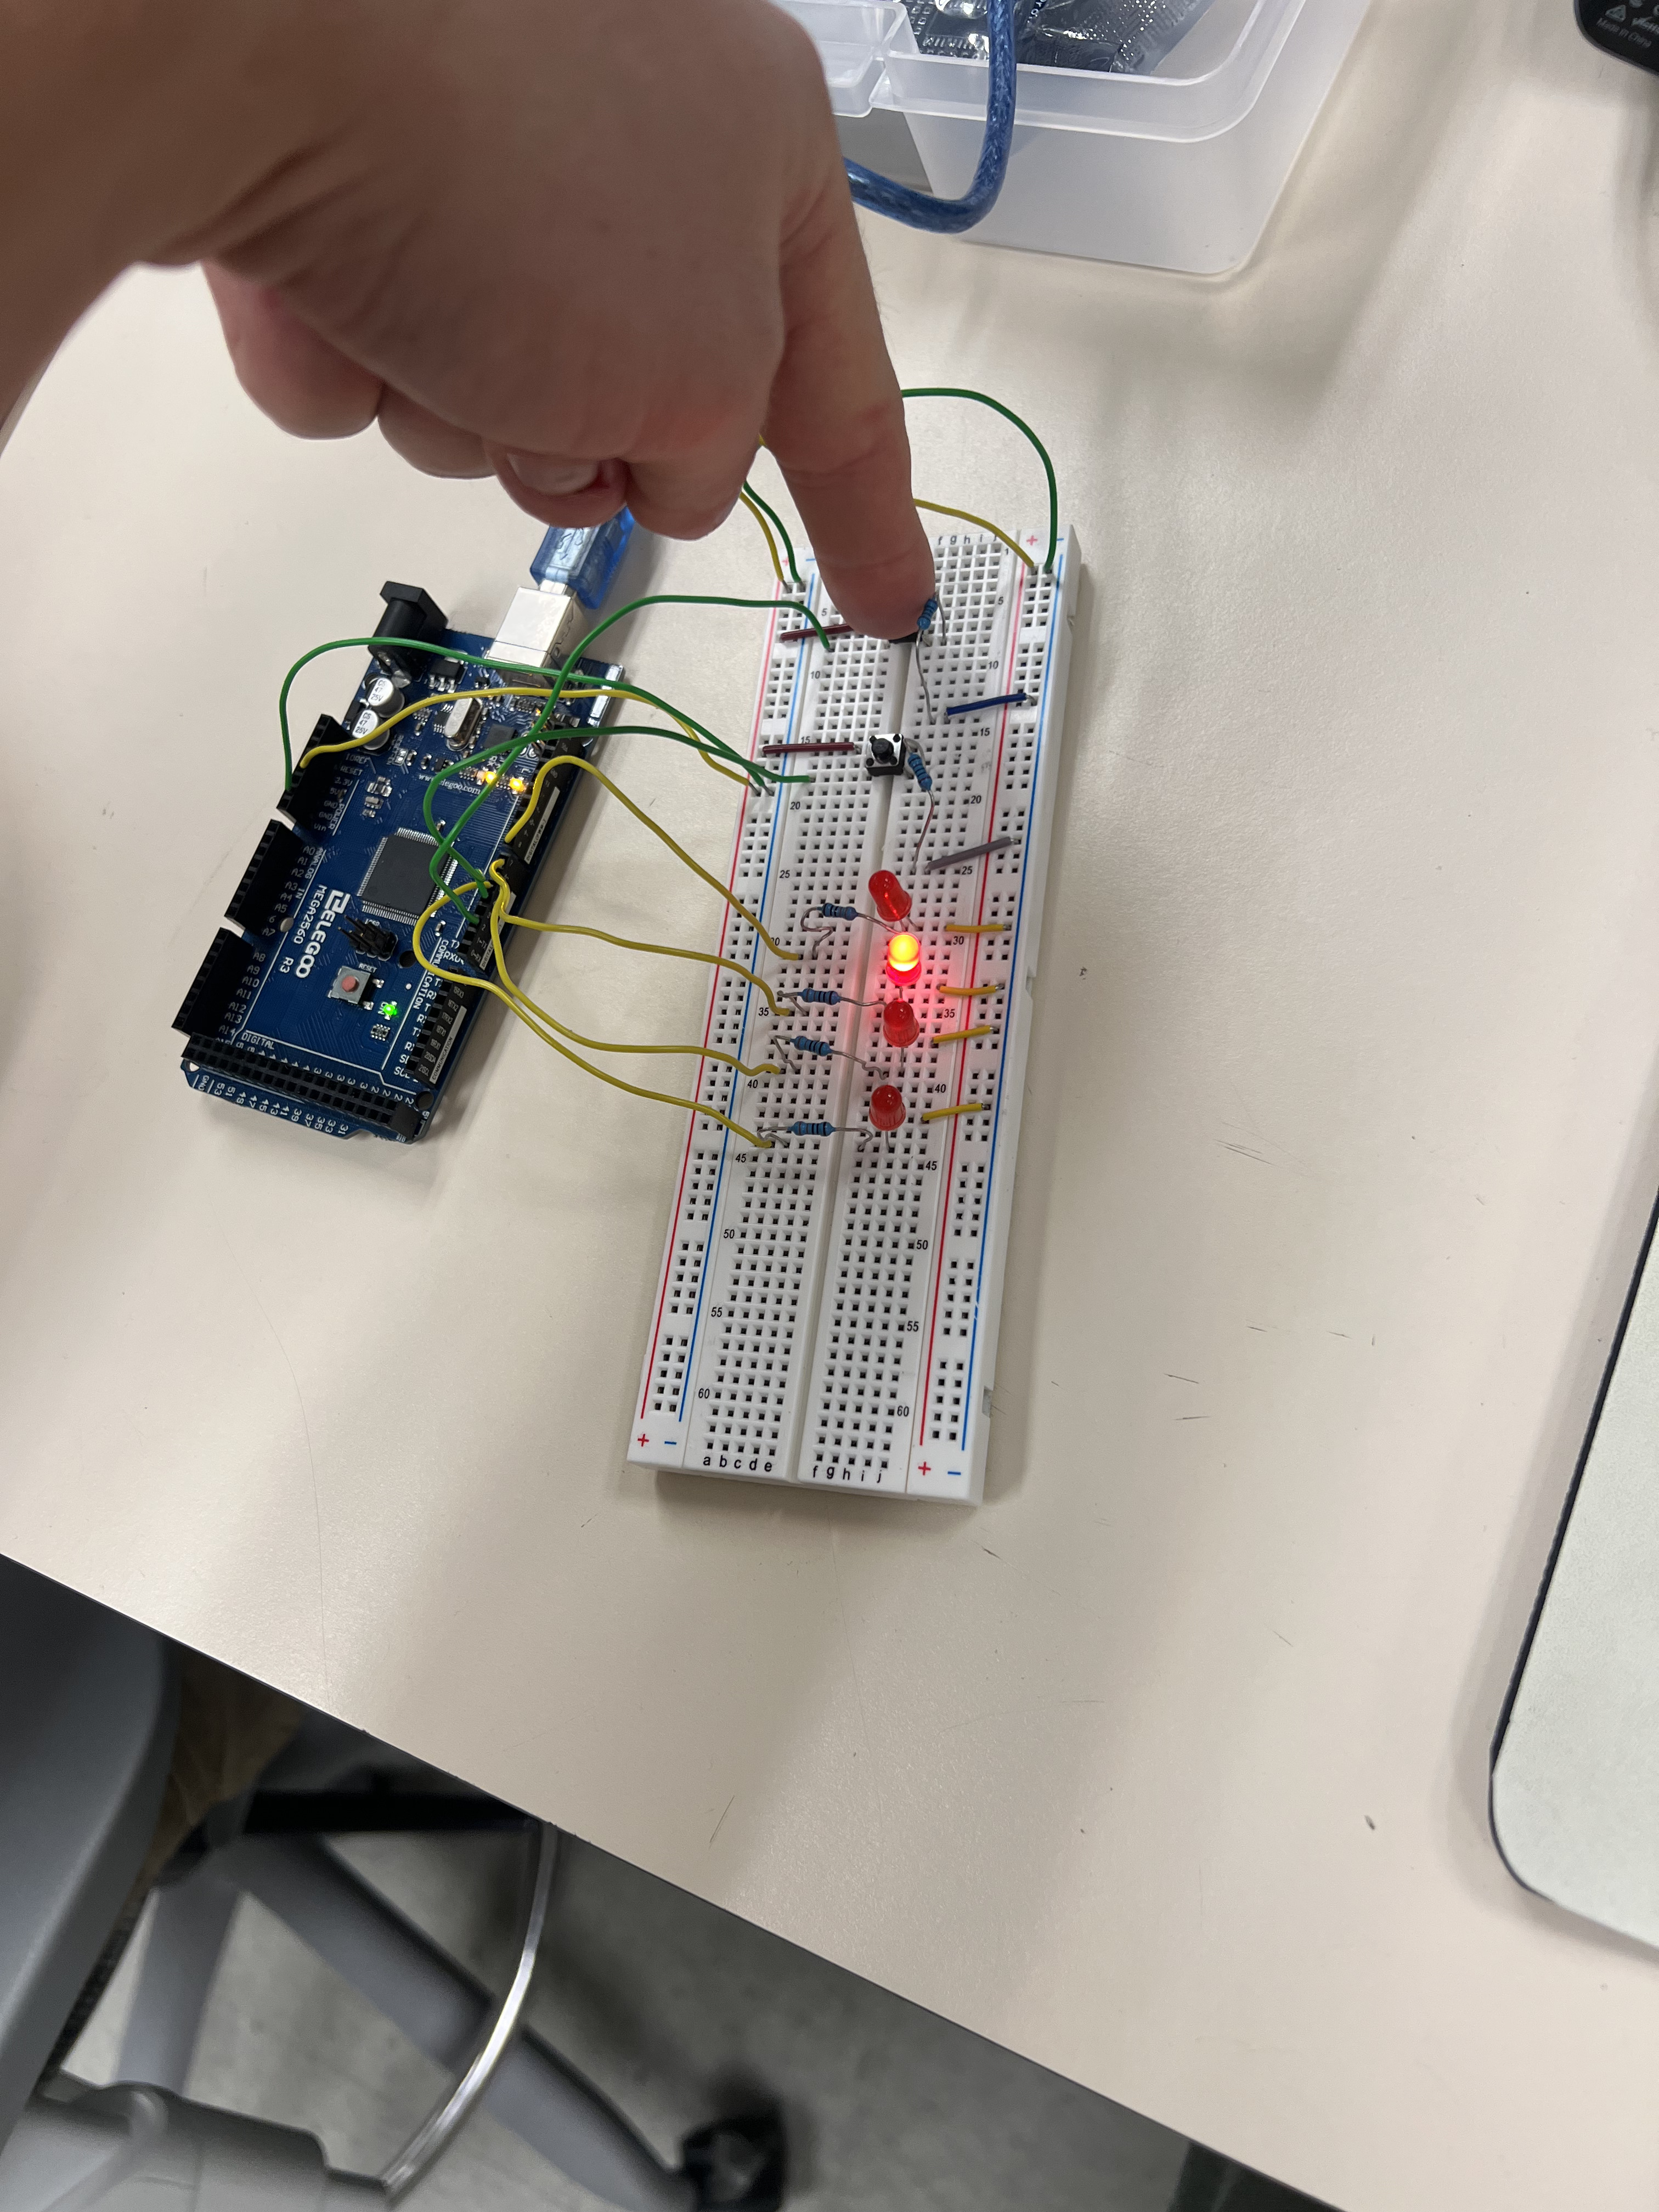
\includegraphics[width=0.28\linewidth]{led-2.jpg}&
            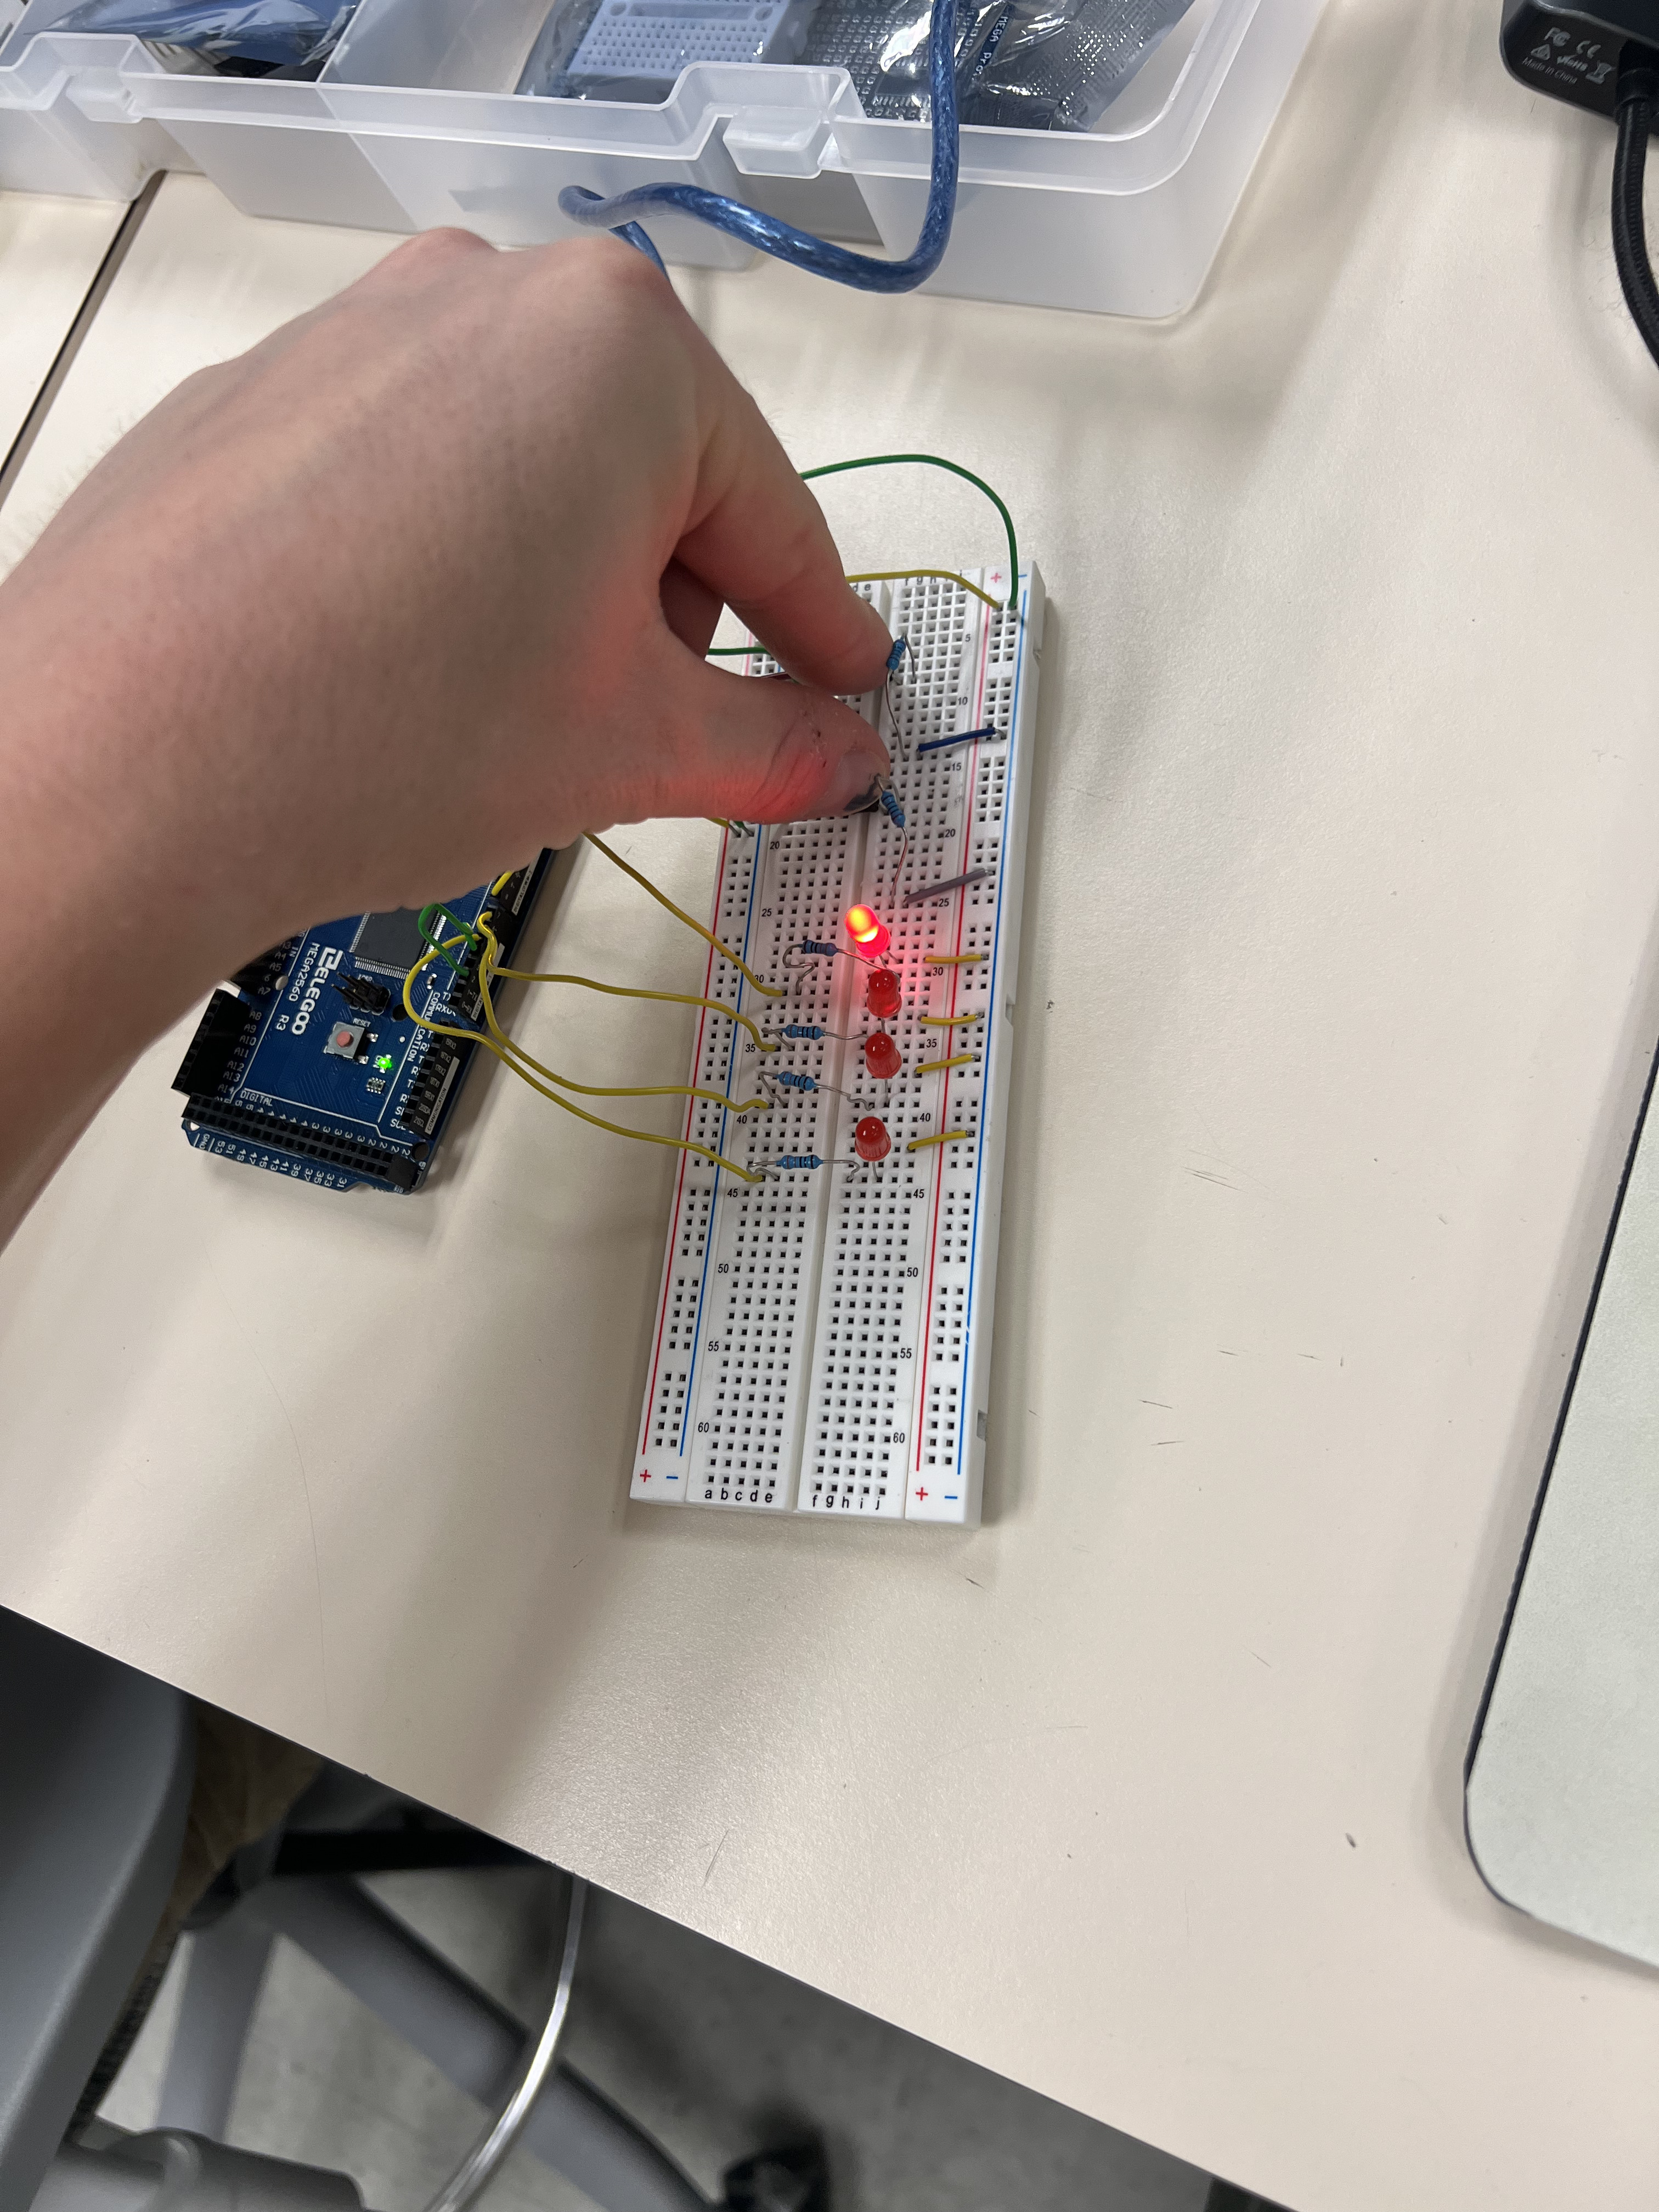
\includegraphics[width=0.28\linewidth]{led-3.jpg} 
            \\
            Button 2 pressed.&
            Both buttons pressed.
            \\
        \hline
    \end{tabular}
    \caption{The various light configurations that result from the circuit.}
    \label{tab:light-configs}
\end{table}

\subsection{Code}

The code was made on Arduino IDE, heavily based on the code included in the lecture slides. The code initializes a serial connection to the computer, as well as two Digital Inputs and four digital outputs before going into it's main loop. In the main loop, the Arduino checks for the sum of the two buttons. If the sum is 0, light LED 1, if the sum is 1, light LED 2, and so on until LED 4. On lighting up an LED, the "LED number" is printed to the serial port.
 
View code on \href{GitHub}{https://github.com/jrkre/cpe-301}.


\end{document}